%=== CHAPTER TWO (2) ===
%=== Literature Review ===

\chapter{Literature Review}
\label{cha:literature}
\begin{spacing}{1.5}
\setlength{\parskip}{0.3in}

Then comes the main part of your work. To lay the ground, there should first be a chapter on what has been done before on the problem - a Literature Review. This is an important section because it shows that you do not narrowly focus only on what you do, but are aware of the
related work elsewhere, some of which might be instructive to your solving the problem. It can also explain why you are taking the direction you do.

\section{An Overview}
\label{sec:LR_overview}

In the past few years, the lane detection method have been developed from classical ones to novel deep-learning based ones. In this section, I will give a brief review of the classical lane detection methods proposed, and also give a brief overview of the developments in the field of object detection.

\subsection{Classical Lane Detection}

There are several ways to get the information for lane detection and prediction usage, such as Monocular vision, stereo, LIDAR, inertial measurement unit (IMU) combined with information obtained from global positioning system (GPS) and high resolution digital maps. \cite{hillel2014recent}. In this work I focus on Monocular vision (Single camera).

In previous work, researchers found relation between wheeling and gaze direction when driving. Human employs the distant region to estimate the road curvature \cite{land1995parts}. Also, the gaze direction relies on the 'tangent point' on the inside of each curve when driving on curvature of the road ahead \cite{land1994we}. This gives possible to utilize the unseen vanishing point in lane prediction.

\subsection{Deep-learning based Lane Detection}

Lane and road marking detection tasks are within the scope of object detection, so algorithms popular in object detection have been implemented in lane detection \cite{tang2020review}. 

Recent years, with the DCNN like AlexNet \cite{krizhevsky2012imagenet} being brought up, deep learning has been driving significant progress in the object detection area. Later RCNN and its variants \cite{girshick2014rich, girshick2015fast, ren2015faster} integrates CNN with the region proposal selective search; GoogLeNet \cite{szegedy2015going} and VGGNet \cite{simonyan2014very} gained improvement with deeper encoder. With the network going deeper, computational efficiency becomes the main problem. More powerful network architectures such as ResNets \cite{he2016deep}, DenseNets \cite{huang2017densely} and Inception \cite{ioffe2015batch} have been proposed, which combine path blocks to reduce the number of parameters while improving the accuracy. Most recently, DETR \cite{carion2020end} combined the CNN with transformer architecture, taking the object detection problem as a set-set mapping and achieved promising results on big-object detection.

Lanes are thin and small objects, thus general methods sometimes work bad \cite{tang2020review}. There are some researches featured in picking out small items. U-Net \cite{ronneberger2015unet} extracts the feature map from encoding path and attach it with the decoding path, by which method the network can keep context for local features.

Efforts to use the neural network in lane detection tasks have also been proved solid. Work \cite{borji2016vanishing} first used the CNN structure to predict the vanishing point, and VPGNet \cite{lee2017vpgnet} employed vanishing point information by multi-task method to enhance the prediction of the lanes.

\section{Neural Network Basis}

Neural Network is the most distinguish deep learning architecture based on Neural units recent years. Compared with conventional machine learning and human-designed mathematical classification algorithms, deep learning on the Neural Network have many advantages. In this section, I will give the theoretical basis of the Neural Networks, and also explain how it works by introducing the back propagation mechanism.

\subsection{Machine Learning}

Compared with specific mathematical equations designed for different kinds of problems, the conventional machine learning are based on \textit{experience}. \textit{Experience} here means that: the machine learning computational models can learn the features from a given data set (learn the \textit{experience} from input), and do prediction or classification based on the that \textit{experience} for any inputs, whether have seen or unseen before.~\cite{mohri2018foundations}.

The process of learning the features can be seen as a clustering operation. Each input data can be mapped into a $n$-dimension vector, and each vector can be viewed as a point in the $n$-dimension hyperspace. \autoref{fig:2dcluster} and \autoref{fig:3dcluster} shows the $2D$ and $3D$ clustering process. Clustering is to group data points into different clusters in the hyperspace, and draw the hyperplane between such clusters. This hyperplane is the interface between classes. For example, in figure \autoref{fig:2dcluster}, 2 groups of data were divided by a linear line, and in figure \autoref{fig:3dcluster}, 2 groups of data were divided by a non-linear curved surface.

\begin{figure}[ht]
\centering
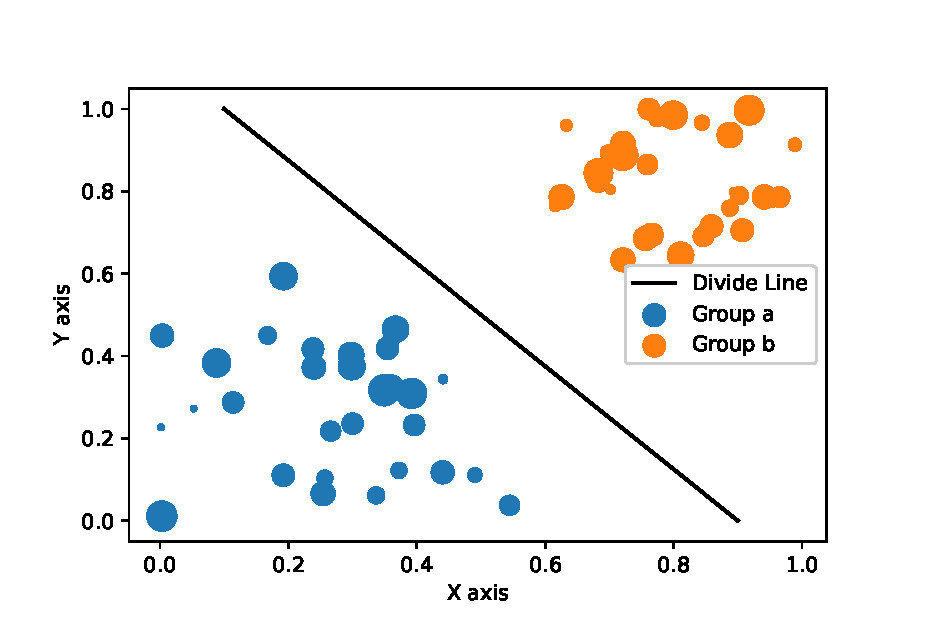
\includegraphics[width=0.99\textwidth, fbox]{Chapter2/2dcluster.eps}
\caption{$2D$ Clustering}
\label{fig:2dcluster} 
\end{figure}

\begin{figure}[ht]
\centering
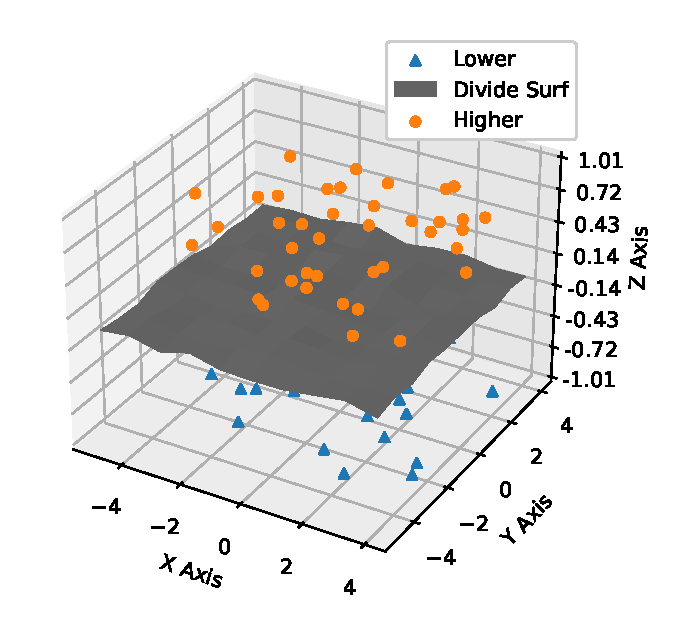
\includegraphics[width=0.6\textwidth, fbox]{Chapter2/3dcluster.eps}
\caption{$3D$ Clustering}
\label{fig:3dcluster} 
\end{figure}

Above mentioned examples only calculate linear or non-linear division between two classes, but normally in real world applications, what needed are not limited to binary classification but usually multi-classification. In the machine learning, there are two solutions on multi-classification problem: 

1) \textit{Uncombined algorithms} will treat the multi-classification as a whole and finish training in only one phase, such as $N$-class SVM, decision trees. 

2) \textit{Aggregated algorithms} will split $N$ class classification into many binary classification, thus need multiple training phase. There are two types of aggregated algorithms: a) \textit{One-versus-one} calculate boundaries for every pair of classes, thus for $N$ class, it needs $N!=N*(N-1)*...*2*1$ calculations, as shown in \autoref{fig:121}. b) \textit{One-versus-others} calculate the boundary between the target class and all other data, thus for $N$ class, it needs to calculate $N$ boundaries, as shown in \autoref{fig:12all}. 

\begin{figure}[th]
    \centering
    \begin{subfigure}[b]{0.49\textwidth}
        \centering
        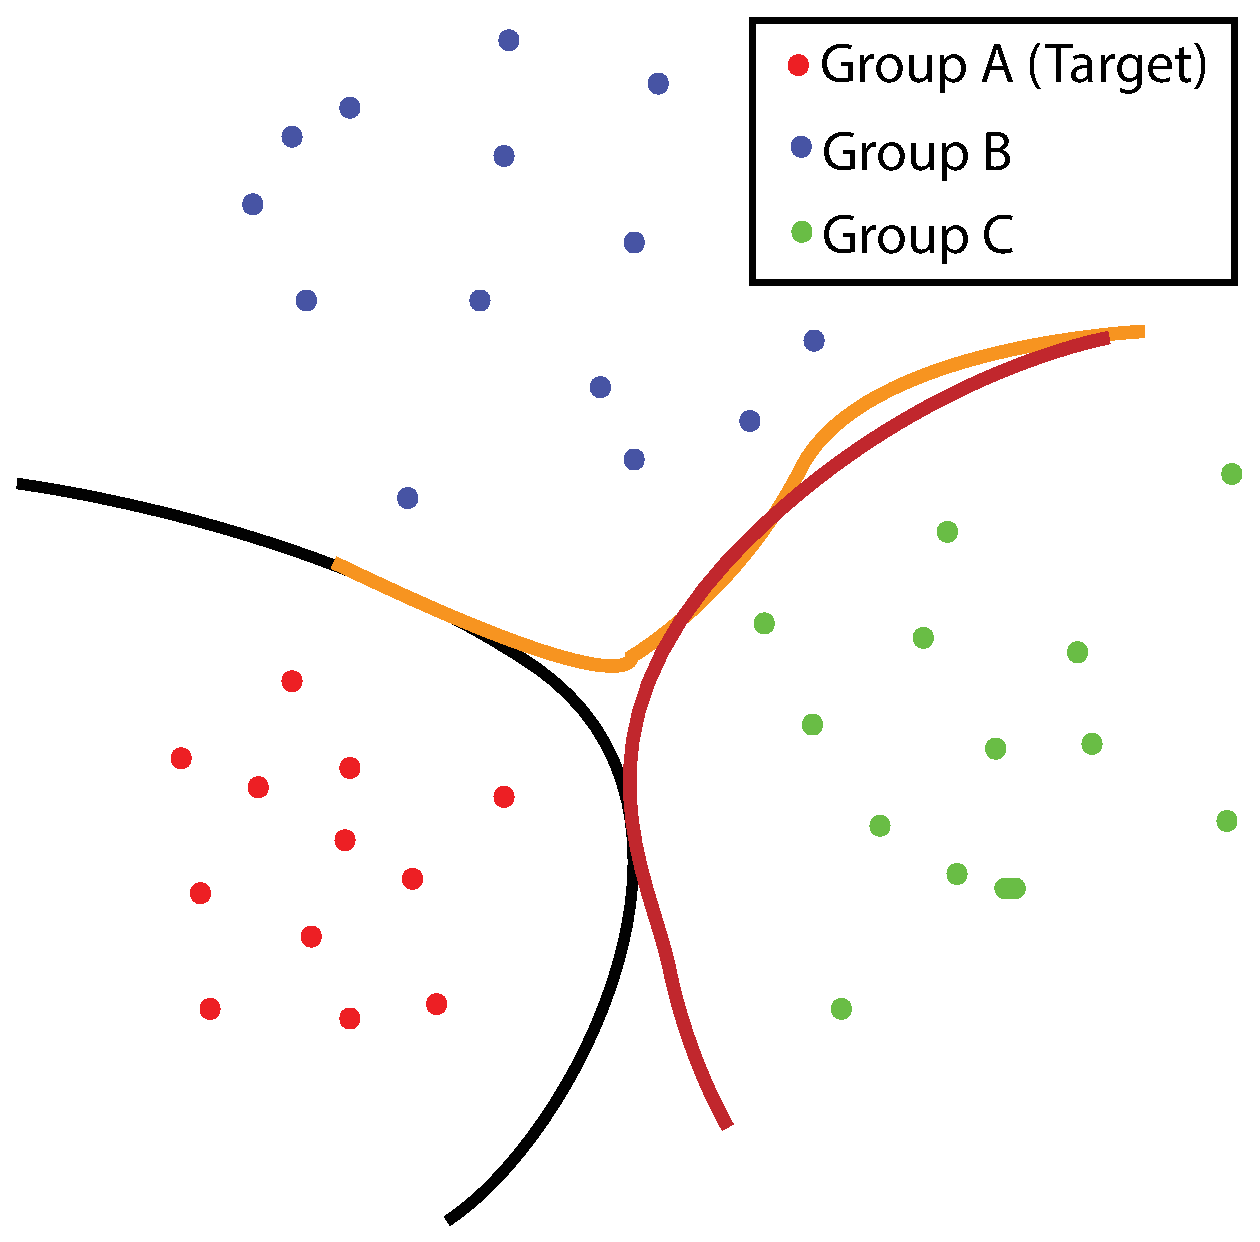
\includegraphics[width=2.7in, fbox]{Chapter2/1to1.eps}
        \caption{One-to-one Multi-classification}
        \label{fig:121} 
    \end{subfigure}%
    ~
    \begin{subfigure}[b]{0.49\textwidth}
        \centering
        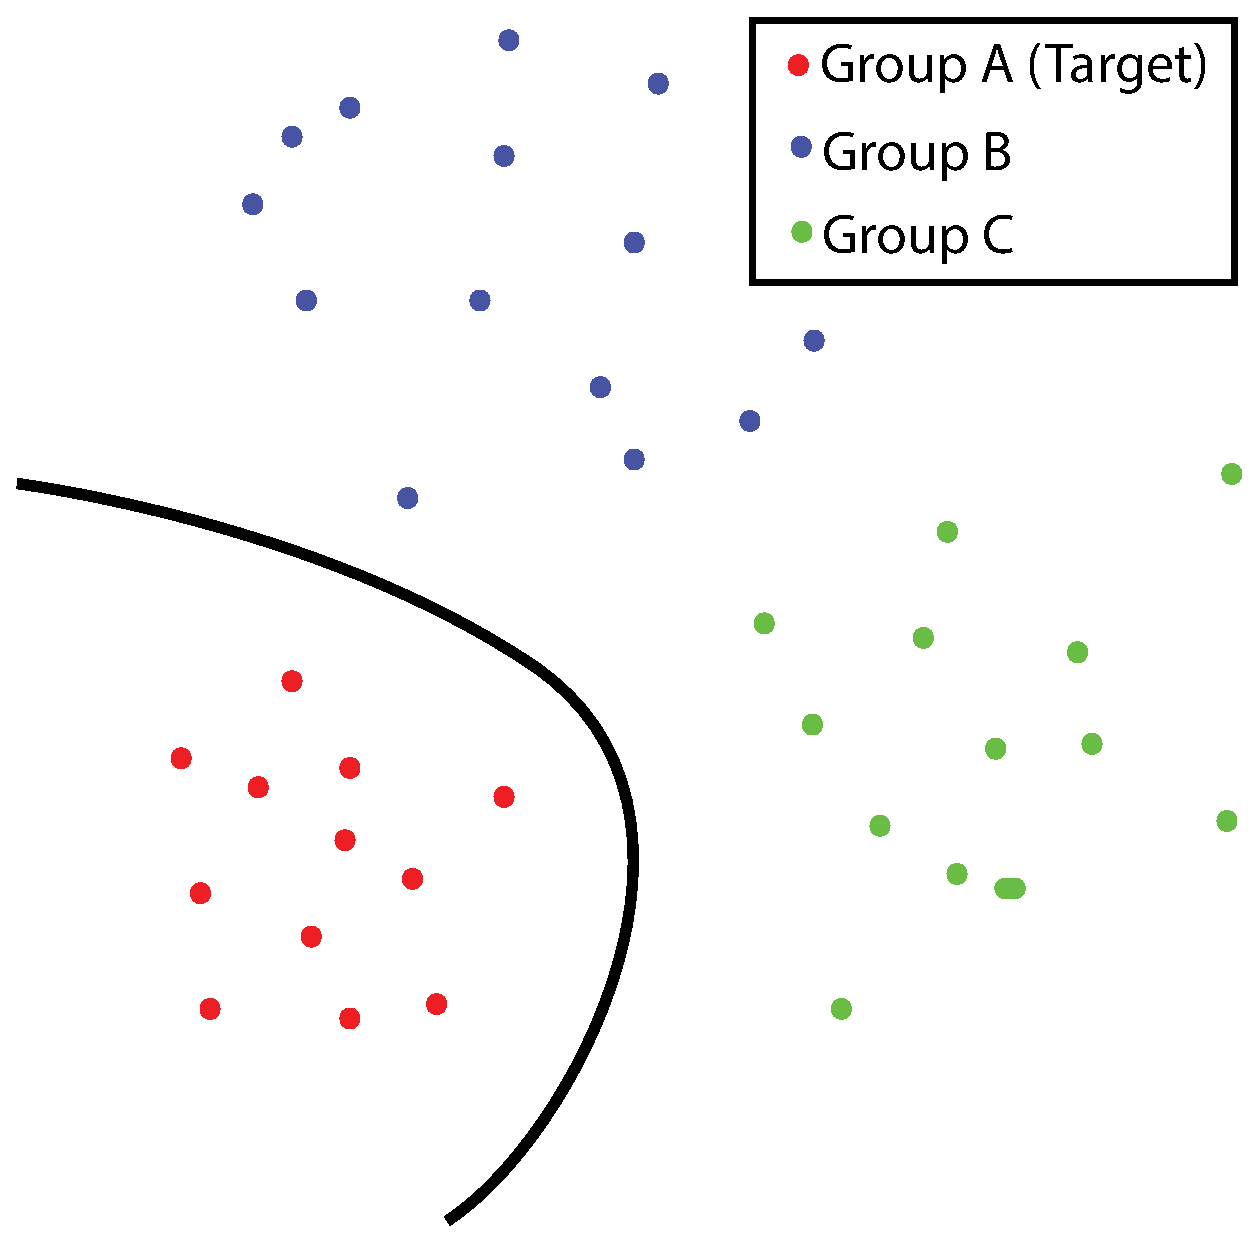
\includegraphics[width=2.7in, fbox]{Chapter2/1toall.eps}
        \caption{One-to-all Multi-classification}
        \label{fig:12all} 
    \end{subfigure}
    \caption{Two Aggregated Algorithms}
\end{figure}


\subsection{Supervised Learning}

\subsection{Neural Unit}

\subsection{Back Propagation and Feedforward Network}

\section{Fully Convolution Networks}
\label{sec:LR_FCN}

\subsection{Convolutional Layer}

\subsection{Convolutional Neural Networks}

\section{Object Detection}
\label{sec:LR_objectdetection}



\section{Vanishing Points in Neural Networks}
\label{sec:LR_vpinNN}



%=== END OF CHAPTER TWO ===
\end{spacing}
\newpage
